\documentclass[a4paper,10pt]{scrartcl}
\usepackage[ngerman]{babel}
\usepackage[T1]{fontenc}
\usepackage[utf8]{inputenc}
\usepackage{graphicx} 

\title{Software Engineering 3}
\author{Benjamin Altmiks}
\date{8. Oktober 2018 - \today}

\begin{document}
\tableofcontents
\maketitle

\section{Einleitung}
\subsection{Rückblick}
        \textbf{Zeit:}      Bei Zeit wird Start und Enddatum/Stunde verwendet. Es ist nicht relevant wie viele Personen an dem Projkt beteiligt waren.
\newline\textbf{Kosten:}    Äquivalent zur Zeit, da die Areitszeit bezahlt werden muss. 
                                Hier ist es relevant wie viele Personen an diese Projekt gearbeitet haben da ealle bezahlt werden müssen.
\newline\textbf{Qualität}:   Unterscheidung zwischen Produktqualität und Prozessqualität.
\begin{itemize}
    \item Produktqualität: Der ganze Prozess, das beeinhaltet Brauchbarkeit und Wartbarkeit 
    \item Prozessqualität: Das Endprodukt, das Ergebniss, das heißt die Software selber
\end{itemize}
\section{Architektur}
\subsection{Allgemein}
\begin{quote}   "Architektur ist schwer greifbar" \newline -Vogel   \end{quote}
Architktur ist ein sich selbst durch die Evolution entwicklender Prozess. Sie ist ein universeller Bestandteil/Grundriss von Software
\begin{quote}    "... werden Entwickler, wenn auch oft unbemerkt, in ihrer täglichen Arbeit mit Architektur konfrontiert, weil diese impliziet immer ein Aspekt von
Software ist und sich nicht eliminieren, allenfalls ignorieren lässt." \newline -Vogel    \end{quote}
\textbf{Softwarearchitektur ist eine strukturierte oder hierarchische Anordnung der Systemkomponenten sowie Beschreibung ihrer Beziehungen. Diese nennt man häufig Architekturmuster}
\newpage
\subsection{Architekturmuster}
Architekturmuster versuchen eine grundlegede Organisation und Interaktion zwischen Komponenten einer Anwendung her zu stellen. Man unterscheidet allgemein Strukturierende Architekturmuster, Muster für Interaktive Systeme und Muster für verteilte Sytsteme

\subsubsection{Strukturierende Architekturmuster}
\textbf{Pipes und Filter}
\begin{itemize}
    \item Beschreibt die Struktur für Systeme, die Datenströme verarbeiten.
    \item Filter = Verarbeitungsschritt mit Dateneingabe und Datenausgabe
    \item Pipes = Verbindung zwischen einzelner Komponenten \newline
    $\Rightarrow$ Verschiedene, unabhängige Komponenten für flexible, unterschiedliche Aufgaben
\end{itemize}
\textbf{Schichten}
\begin{itemize}
    \item Aufteilung auf Schichten für große/komplexe Systeme 
    \item Ziel ist eine Abhängigkeitslösung der Komponenten zu erreichen\newline
    $\Rightarrow$ Austauschbarkeit und Integration neuer Systeme einfacher möglich
    \item Ein Besipiel ist das OSI-Schichtenmodell bei Netzwerkprotokollen
\end{itemize}
\subsubsection{Architekturmuster für interaktive Systeme}
\textbf{Model-View-Controller}\newline
Einteilung in drei Komponenten:
\begin{enumerate}
    \item Datenmodell (model): Enthält die Daten die dargestellt werden. Ist unabhängig von anderens
    \item Präsentation (view): Darstellung der Daten des Modells mit Benutzerinteraktion
    \item Programmsteuerung (controller): Benutzerinteraktionen verwaltet Präsentation und Datenmodell
\end{enumerate}
$\Rightarrow$ Reduzierung von Abhängigkeiten, Benutzerschnittstellenorientiert  \newline
\begin{figure}[h]
	\centering
	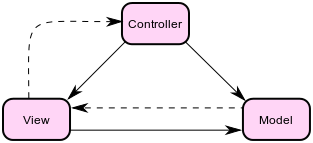
\includegraphics[width = 4.5cm]{ModelViewControllerDiagram2}
\end{figure}
\newpage
\subsubsection{Architekturmuster für verteilte Systeme}
\textbf{Vermittler-Prinzip}

\begin{itemize}
    \item Verteiltes System mit (unabhängigen) Komponenten, die zusammenarbeiten 
    \item Vermittler steuert Objekte, Objekte nicht untereinander\newline
    $\Rightarrow$ Einfache Kombination von Diensten und Objekten in einem System
\end{itemize}
\textbf{Client-Server}
\begin{itemize}
    \item Verteilte Benutzer mit zentraler Anwendung 
    \item Verschiedene Funktionalitäten durch Verteilung auf Netzwerkkomponenten\newline
    $\Rightarrow$ Beispiele sind das WWW oder E-Mail 
\end{itemize}
\subsubsection{Zusammenfassung}
\begin{itemize}
    \item Architektur bringt keinen direkten Mehrwert für die Software mit sich
    \item Funktionale Zusätzliche Fähigkeiten und Flexibilität der Software besser\newline
    $\Rightarrow$ Zukunftssichere Software (Kostengünstiger, Zuverlässiger)
    \item Gute Architektur ist eine notwendige, aber keine hinreichende Voraussetzung für gute Qualität
\end{itemize}
\end{document}
